\section{Simulation study}

We utilize a simulation study to highlight the utility of AME as an inferential tool for dyadic analysis. The goal of the simulation is to assess how well AME can provide unbiased and well calibrated estimates of coefficient parameters in the presence of unobserved dependencies. Specifically, we are concerned with conducting inference on a regression parameter $\beta$ of a linear model for a network in the case where there is an omitted variable. Say that the true data-generating process for a particular $Y$ is given by:

\begin{align*}
	y_{i,j} \sim  \mu + \beta x_{i,j} + \gamma w_{i,j} + \epsilon_{i,j} \\
	\label{eqn:sim}
\end{align*}

where $Y= \{y_{i,j}\}\in \mathbb R^{n\times n}$ is an observed sociomatix, $x = \{x_{i,j} \} \in \mathbb R^{n \times n}$ is a matrix of observed dyad-specific characteristics, and $w = \{ w_{i,j}\} \in \mathbb R^{n \times n}$ is a matrix of unobserved dyad-specific characteristics. We compare inference for $\beta$ using three models:

\begin{itemize}
	\item the standard IR approach assuming independent errors; 
	\item the AME approach outlined in the previous section with a unidimensional latent factor space ($K=1$);
	\item and an ``oracle'' regression model that includes both $x_{i,j}$ and $w_{i,j}$. 
\end{itemize}

We vary the size of the network under study at 50 and 100.

\begin{figure}
	\centering
	\caption{Bias in parameter when homophily is ignored.}
	\label{fig:ameBias}
	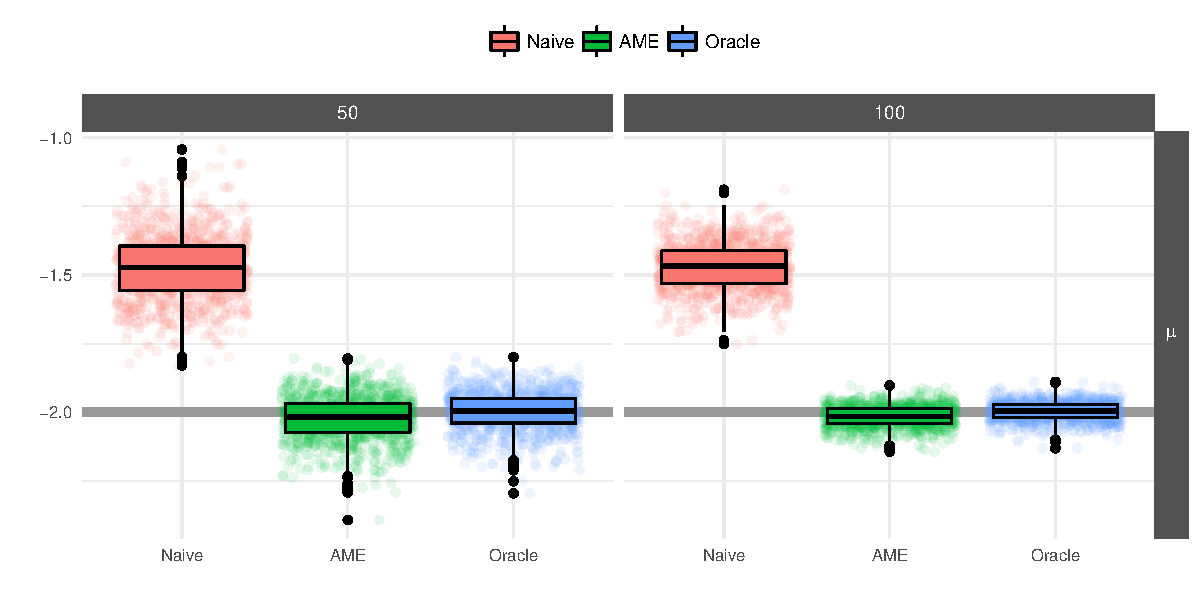
\includegraphics[width=1\textwidth]{ameSimBias_mu.pdf} \\
	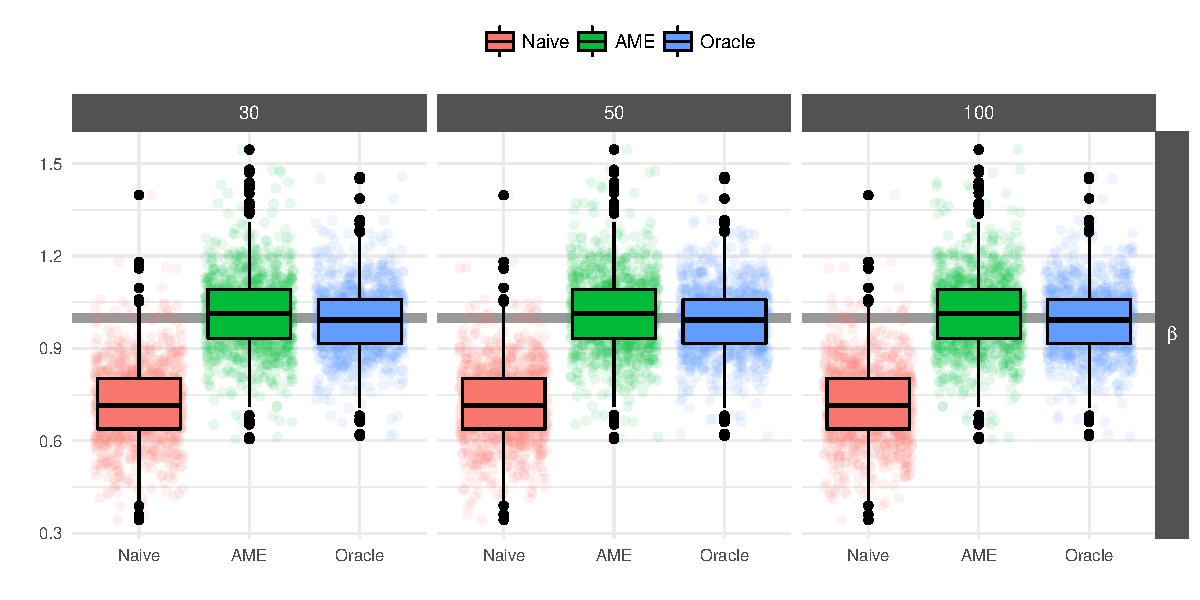
\includegraphics[width=1\textwidth]{ameSimBias_beta.pdf}
\end{figure}

One way to compare inferences across models is  with bias and variance of the parameter estimates. Both of these quantities are combined to get the MSE. 

\begin{figure}
	\centering
	\caption{Coverage in parameter when homophily is ignored.}
	\label{fig:ameCalib}
	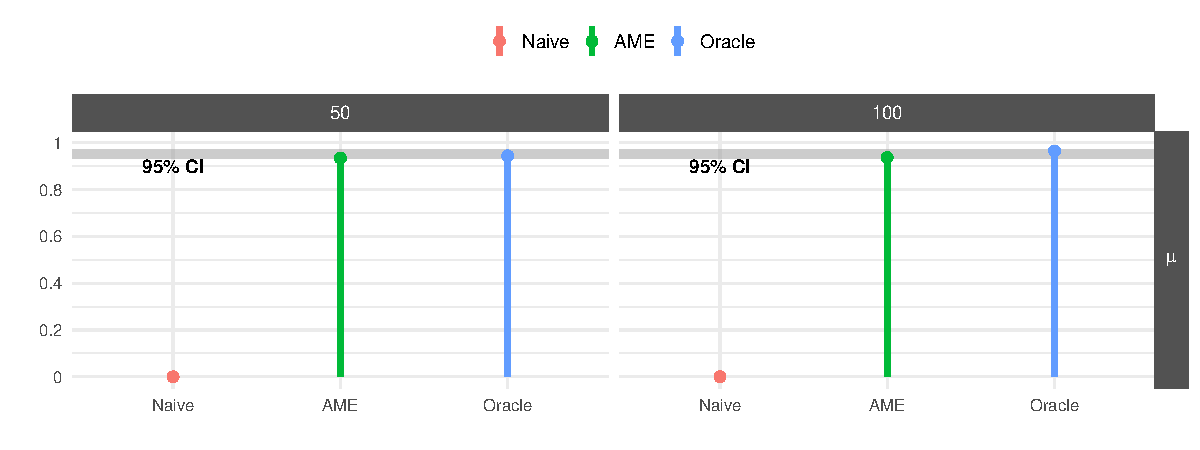
\includegraphics[width=1\textwidth]{ameSimCover_mu.pdf} \\
	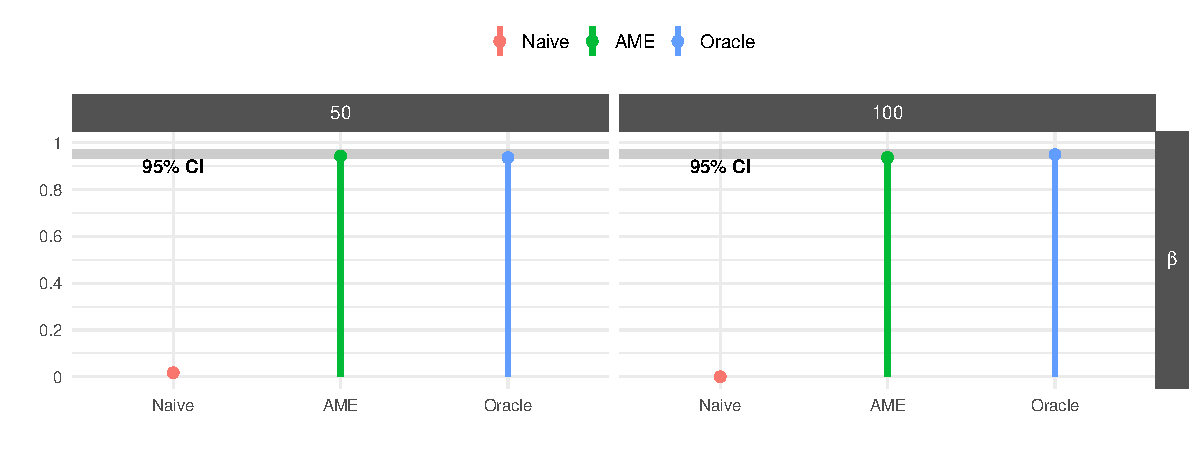
\includegraphics[width=1\textwidth]{ameSimCover_beta.pdf}
\end{figure}

Alternatively, bias and precision can be summarized by confidence interval coverage and width. Coverage should ideally be at the nominal level. If two methods have the same actual coverage rate, the one with the narrower intervals is preferred. 

\begin{figure}
	\centering
	\caption{Correlation between missing variable and multiplicative random effect in AME.}
	\label{fig:ameCorr}
	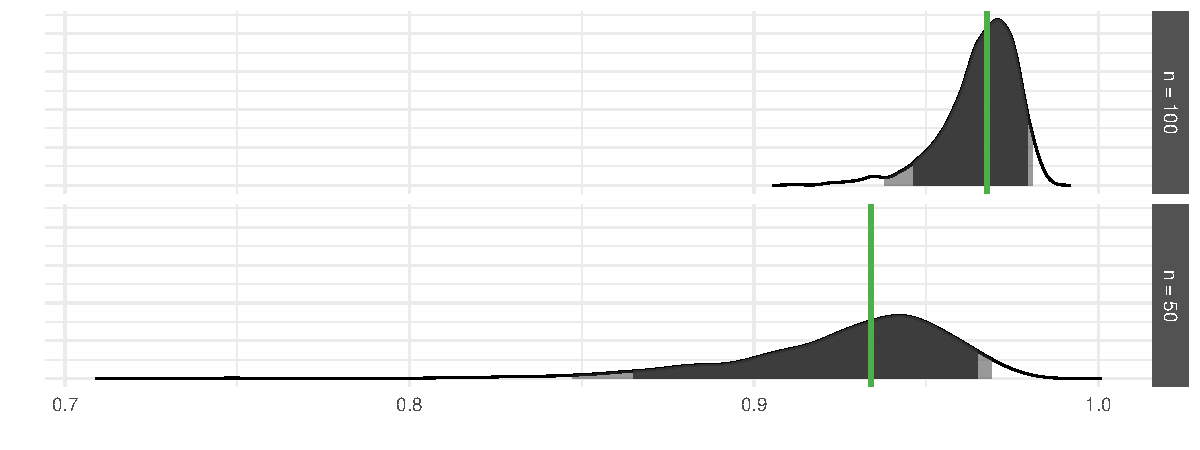
\includegraphics[width=1\textwidth]{ameSimCorr.pdf} \\
\end{figure}
